\section{Results}\label{sec:results}
For our experiments, we used a Red Hat 8 server with a Intel Xeon Gold 6242
CPU. Since \shortname{} is written in Rust, it mostly uses the built-in
functionality of the egg library. The egg e-graph runner was ran in a
time-limited configuration, meaning there was no limit in the size of the
e-graph or number of rewrite iterations. The specific time limit for e-graph
construction was 10 minutes. In most cases, the test circuit saturated the
e-graph before this time limit. \shortname{} was evaluated against circuits
from three benchmark suites: EPFL~\cite{epflbench}, ISCAS'85~\cite{iscasbench},
and LGSynth'91~\cite{lgsynthbench}. However, we also included an ALU and
pipelined multiplication module to test how our compiler behaves with
increasing levels of bit-parallelism and pipeline stages. Finally, we measure
how our mapping optimizations influence timing closure.

\subsection{Benchmarking}\label{sec:results:benchmark}
\begin{table}
    \centering
    \csvautobooktabular{data/results.csv}
    \caption{Results of 30 improved benchmarks from ISCAS'85, LGSynth'91, and EPFL}\label{tab:results}
\end{table}
Among the 96 benchmarks we tested, we found that \shortname{} was able to
reduce the LUT count \fmetric{} of the time. On average, \shortname{} packed the
netlists to \metric{}. The results in Table~\ref{tab:results} list the LUT counts \todo{explain table}.

\subsection{Marginal Improvement and Time Cost}\label{sec:results:margin}
\begin{figure}
    \begin{subfigure}{0.47\textwidth}
        \centering
        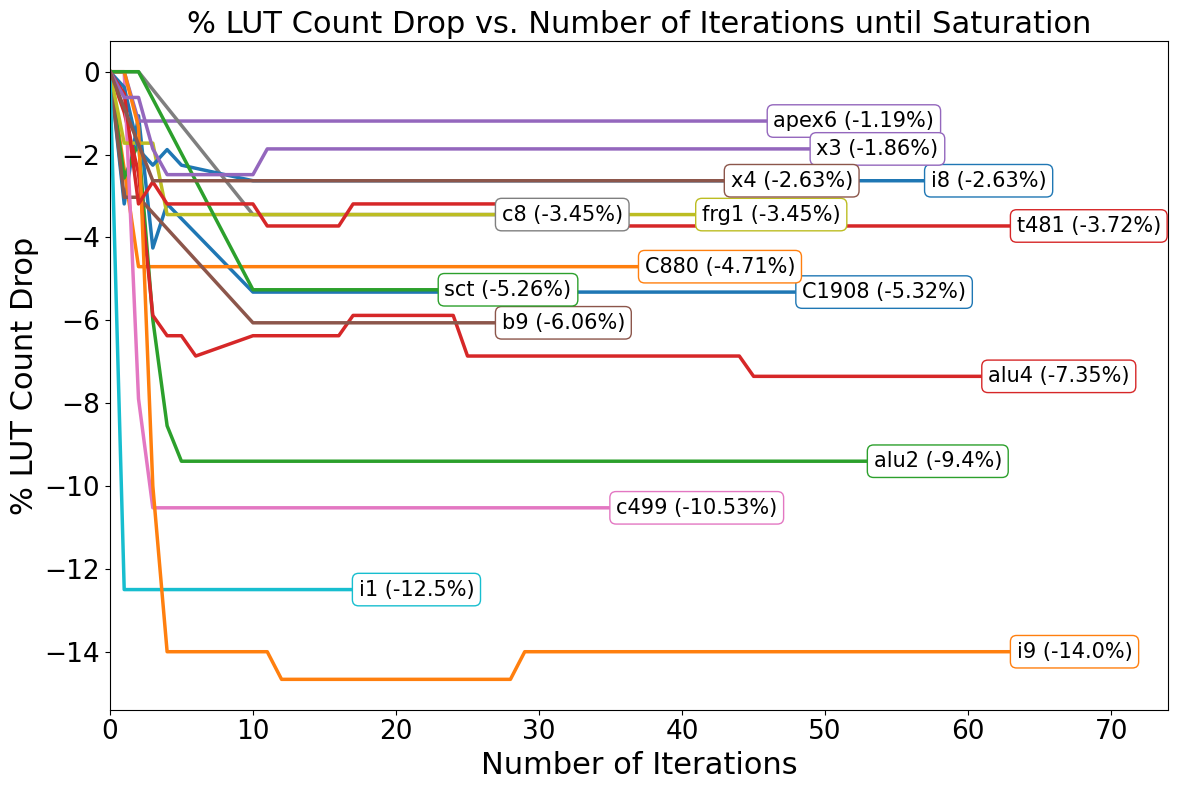
\includegraphics[width=\textwidth]{img/improvement.png}
        \caption{Marginal improvement versus iteration count. The labels mark the equality saturation point.}\label{fig:marginal:improvement}
        \Description[]{}
    \end{subfigure}
    \hfill\vspace{4mm}
    \begin{subfigure}{0.47\textwidth}
        \centering
        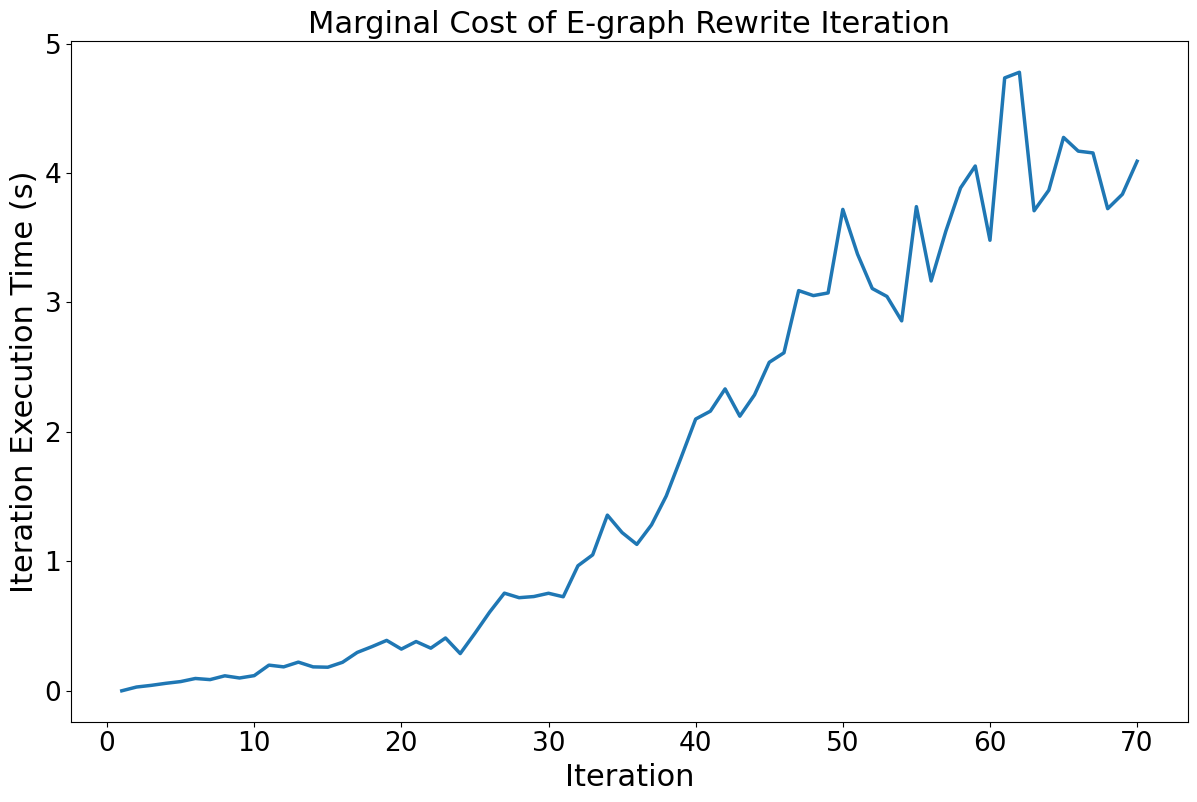
\includegraphics[width=\textwidth]{img/runtime_derivative.png}
        \caption{Marginal increase in runtime versus iteration count. Longer iterations consume more time as the graph is larger.}\label{fig:marginal:runtime}
        \Description[]{}
    \end{subfigure}
    \caption{Comparison between gains in QoR against increasing execution time with graph size. Running a netlist to equality saturation requires more rewrite iterations, and hence a larger e-graph.}\label{fig:marginal}
    \Description[]{}
\end{figure}
\todo{explain graph showing improvement with iter count}

\subsection{Case Study: Pipelined Designs}\label{sec:results:retiming}
\begin{table*}[t]
    \centering
    \csvautobooktabular{data/mult.csv}
    \caption{\todo{mult captiofn}}\label{tab:multiply}
\end{table*}
\todo{explain pipelined mult design}

\subsection{Case Study: Bit-Parallel Designs}\label{sec:results:scalability}
\begin{table}
    \centering
    \csvautobooktabular{data/alu.csv}
    \caption{Synthesis results of $n$-bit ALU}\label{tab:alu}
\end{table}
\todo{explain increasing ALU bit parallelism}
